\documentclass[compsoc]{IEEEtran}
\usepackage{graphicx}
\usepackage{amsmath}
\usepackage{authblk}
\usepackage[english]{babel}
\usepackage{blindtext}
%\usepackage[ruled,vlined,linesnumbered]{algorithm2e}
%\usepackage{algorithmic,float}
\usepackage{setspace}
\usepackage{amsfonts}
%\usepackage{hyperref}
\graphicspath{ {./images/} }
\usepackage{subfig}
\usepackage{fontspec}
\usepackage{listings}
\usepackage{amsmath}
\usepackage{mathabx}
\usepackage[bottom]{footmisc}
\newfontfamily\listingsfont[Scale=.7]{inconsolata}\usepackage[font=footnotesize,labelfont=bf]{caption}
%\captionsetup[algorithm2e]{font=footnotesize}
\usepackage[table,xcdraw]{xcolor}
\usepackage[utf8]{inputenc}
\title{Assignment: CNN and MNIST}
\author{David Bertoldi -- 735213 \\ email: d.bertoldi@campus.unimib.it}
\affil{Department of Informatics, Systems and Communication}
\affil{University of Milano-Bicocca}
\date{October 2022}


\begin{document}

\maketitle 



\section{Inspecting the data}\label{sec:insp}
The MNIST dataset contains $70\,000 $images of handwritten digits ($0$ to $9$) that have been size-normalized and centered in a square grid of pixels. Each image is a $28 \times 28$ array of floating-point numbers representing grayscale intensities ranging from $0$ (black) to $255$ (white). \par
The labels consist of a vector of values, corresponding to the digit classification categories $0$ through $9$. \par
The dataset is already divided into training and test sets, respectively with $60\,000$ and $10\,000$ samples. \par

Figure \ref{fig:data} shows an example of the
population.

\begin{figure}[ht!]
\centering                                                                        
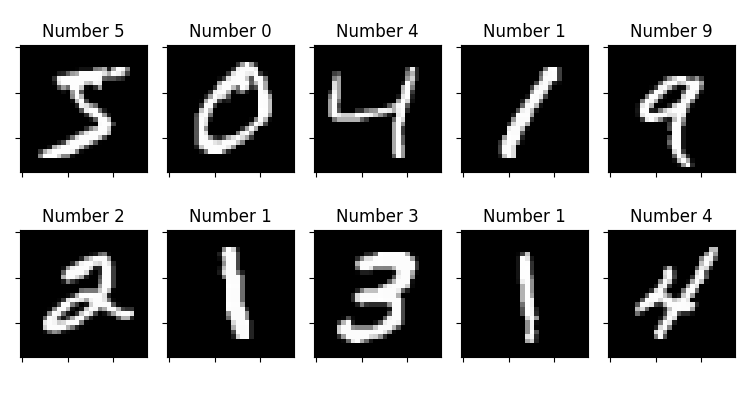
\includegraphics[width=2.5in]{data.png}
\captionsetup{justification=centering}                                                                                         
\caption{The first 10 samples of the train dataset}
\label{fig:data}                                                                                                                               
\end{figure}




The training population presents a distribution with mean $\mu = 6\,000$ and standard deviation $\sigma \simeq 340$ and thus we didn't notice any important unbalance in the data. For this reason we assumed the data followed a distribution $X \sim U(\mu, \sigma)$ and no data augmentation on less populated classes was taken into account. Figure \ref{fig:hist} shows the data distribution for both training and test datasets.

\begin{figure}[ht!]
\centering                                                                        
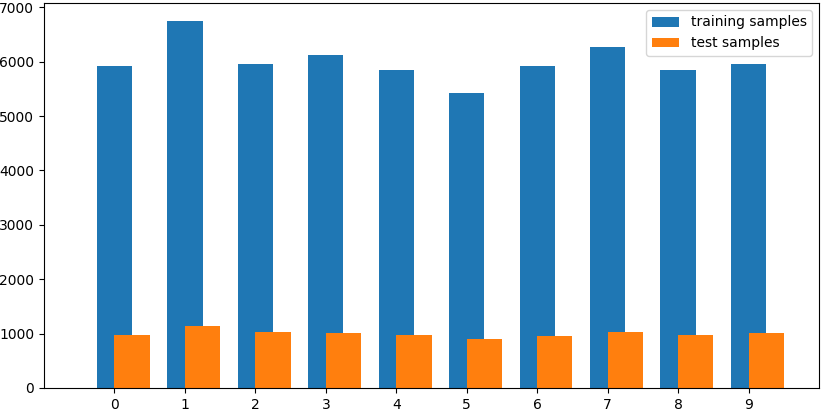
\includegraphics[width=3.5in]{hist.png}
\captionsetup{justification=centering}                                                                                         
\caption{Histogram of the frequency of samples in the dataset}
\label{fig:hist}                                                                                                                               
\end{figure}

\section{Preparing the data}
Before training a FFNN using this images, encoded in $28\times28$ matrices with values from $0$ to $255$, we flattened them in
arrays $1\times784$ and rescaled each value in the continuous interval $[0, 1]$. This encoding will be used in every section of this work: a flat array
better suits the input layer of a FFNN and small values increases the efficiency in the calculations.


\subsection{Data split}
As noted in section \ref{sec:insp}, the dataset is divided into training and test samples. A validation subset is missing and thus
is retrieved from the training set: $15\%$ of the images are randomly used for validation instead of training (along with their labels) for a total of $9\,000$ samples. \par
About labels, we encoded them in one-hot vectors so that the $1$s are set in the index representing the numerical class. \par

\section{Building the network and training}
The aim of this section is to describe a CNN with less than $10\,000$ parameters that is able to classify
with high level of accuracy the numbers from the dataset with or without any regularization technique. 

\subsection{The network}

\begin{figure}[ht!]
\centering                                                                        
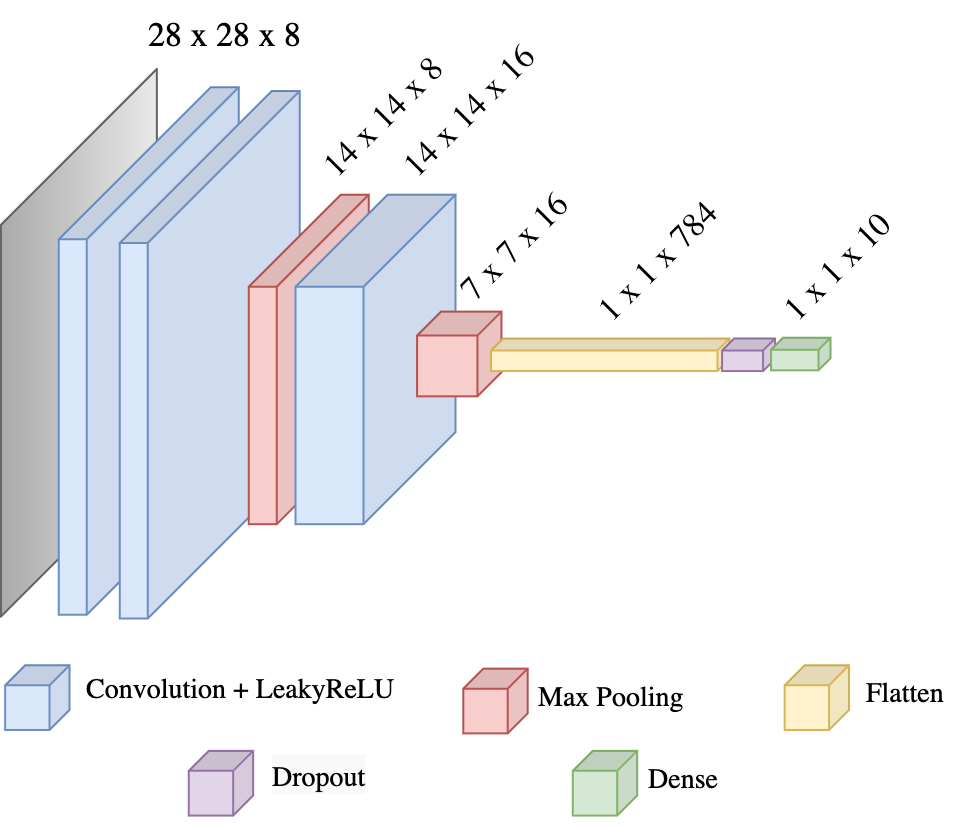
\includegraphics[width=3.5in]{cnn.png}
\captionsetup{justification=centering}                                                                                         
\caption{Histogram of the frequency of samples in the dataset}
\label{fig:cnn}                                                                                                                               
\end{figure}


\end{document}









